
%% bare_jrnl.tex
%% V1.4
%% 2012/12/27
%% by Michael Shell
%% see http://www.michaelshell.org/
%% for current contact information.
%%
%% This is a skeleton file demonstrating the use of IEEEtran.cls
%% (requires IEEEtran.cls version 1.8 or later) with an IEEE journal paper.
%%
%% Support sites:
%% http://www.michaelshell.org/tex/ieeetran/
%% http://www.ctan.org/tex-archive/macros/latex/contrib/IEEEtran/
%% and
%% http://www.ieee.org/



% *** Authors should verify (and, if needed, correct) their LaTeX system  ***
% *** with the testflow diagnostic prior to trusting their LaTeX platform ***
% *** with production work. IEEE's font choices can trigger bugs that do  ***
% *** not appear when using other class files.                            ***
% The testflow support page is at:
% http://www.michaelshell.org/tex/testflow/


%%*************************************************************************
%% Legal Notice:
%% This code is offered as-is without any warranty either expressed or
%% implied; without even the implied warranty of MERCHANTABILITY or
%% FITNESS FOR A PARTICULAR PURPOSE! 
%% User assumes all risk.
%% In no event shall IEEE or any contributor to this code be liable for
%% any damages or losses, including, but not limited to, incidental,
%% consequential, or any other damages, resulting from the use or misuse
%% of any information contained here.
%%
%% All comments are the opinions of their respective authors and are not
%% necessarily endorsed by the IEEE.
%%
%% This work is distributed under the LaTeX Project Public License (LPPL)
%% ( http://www.latex-project.org/ ) version 1.3, and may be freely used,
%% distributed and modified. A copy of the LPPL, version 1.3, is included
%% in the base LaTeX documentation of all distributions of LaTeX released
%% 2003/12/01 or later.
%% Retain all contribution notices and credits.
%% ** Modified files should be clearly indicated as such, including  **
%% ** renaming them and changing author support contact information. **
%%
%% File list of work: IEEEtran.cls, IEEEtran_HOWTO.pdf, bare_adv.tex,
%%                    bare_conf.tex, bare_jrnl.tex, bare_jrnl_compsoc.tex,
%%                    bare_jrnl_transmag.tex
%%*************************************************************************

% Note that the a4paper option is mainly intended so that authors in
% countries using A4 can easily print to A4 and see how their papers will
% look in print - the typesetting of the document will not typically be
% affected with changes in paper size (but the bottom and side margins will).
% Use the testflow package mentioned above to verify correct handling of
% both paper sizes by the user's LaTeX system.
%
% Also note that the "draftcls" or "draftclsnofoot", not "draft", option
% should be used if it is desired that the figures are to be displayed in
% draft mode.
%
\documentclass[journal]{IEEEtran}
%
% If IEEEtran.cls has not been installed into the LaTeX system files,
% manually specify the path to it like:
% \documentclass[journal]{../sty/IEEEtran}


\usepackage{eurosym}


% Some very useful LaTeX packages include:
% (uncomment the ones you want to load)


% *** MISC UTILITY PACKAGES ***
%
%\usepackage{ifpdf}
% Heiko Oberdiek's ifpdf.sty is very useful if you need conditional
% compilation based on whether the output is pdf or dvi.
% usage:
% \ifpdf
%   % pdf code
% \else
%   % dvi code
% \fi
% The latest version of ifpdf.sty can be obtained from:
% http://www.ctan.org/tex-archive/macros/latex/contrib/oberdiek/
% Also, note that IEEEtran.cls V1.7 and later provides a builtin
% \ifCLASSINFOpdf conditional that works the same way.
% When switching from latex to pdflatex and vice-versa, the compiler may
% have to be run twice to clear warning/error messages.






% *** CITATION PACKAGES ***
%
%\usepackage{cite}
% cite.sty was written by Donald Arseneau
% V1.6 and later of IEEEtran pre-defines the format of the cite.sty package
% \cite{} output to follow that of IEEE. Loading the cite package will
% result in citation numbers being automatically sorted and properly
% "compressed/ranged". e.g., [1], [9], [2], [7], [5], [6] without using
% cite.sty will become [1], [2], [5]--[7], [9] using cite.sty. cite.sty's
% \cite will automatically add leading space, if needed. Use cite.sty's
% noadjust option (cite.sty V3.8 and later) if you want to turn this off
% such as if a citation ever needs to be enclosed in parenthesis.
% cite.sty is already installed on most LaTeX systems. Be sure and use
% version 4.0 (2003-05-27) and later if using hyperref.sty. cite.sty does
% not currently provide for hyperlinked citations.
% The latest version can be obtained at:
% http://www.ctan.org/tex-archive/macros/latex/contrib/cite/
% The documentation is contained in the cite.sty file itself.






% *** GRAPHICS RELATED PACKAGES ***
%
\ifCLASSINFOpdf
  \usepackage[pdftex]{graphicx}
  % declare the path(s) where your graphic files are
  %\graphicspath{{../pdf/}{../jpeg/}}
  % and their extensions so you won't have to specify these with
  % every instance of \includegraphics
  \DeclareGraphicsExtensions{.pdf,.jpeg,.png}
\else
  % or other class option (dvipsone, dvipdf, if not using dvips). graphicx
  % will default to the driver specified in the system graphics.cfg if no
  % driver is specified.
  \usepackage[dvips]{graphicx}
  % declare the path(s) where your graphic files are
  % \graphicspath{{../eps/}}
  % and their extensions so you won't have to specify these with
  % every instance of \includegraphics
  % \DeclareGraphicsExtensions{.eps}
\fi
% graphicx was written by David Carlisle and Sebastian Rahtz. It is
% required if you want graphics, photos, etc. graphicx.sty is already
% installed on most LaTeX systems. The latest version and documentation
% can be obtained at: 
% http://www.ctan.org/tex-archive/macros/latex/required/graphics/
% Another good source of documentation is "Using Imported Graphics in
% LaTeX2e" by Keith Reckdahl which can be found at:
% http://www.ctan.org/tex-archive/info/epslatex/
%
% latex, and pdflatex in dvi mode, support graphics in encapsulated
% postscript (.eps) format. pdflatex in pdf mode supports graphics
% in .pdf, .jpeg, .png and .mps (metapost) formats. Users should ensure
% that all non-photo figures use a vector format (.eps, .pdf, .mps) and
% not a bitmapped formats (.jpeg, .png). IEEE frowns on bitmapped formats
% which can result in "jaggedy"/blurry rendering of lines and letters as
% well as large increases in file sizes.
%
% You can find documentation about the pdfTeX application at:
% http://www.tug.org/applications/pdftexhttps://www.google.be/search?q=or+no&ie=utf-8&oe=utf-8&aq=t&rls=org.mozilla:en-US:official&client=firefox-a&gfe_rd=cr&ei=w3x8U6meBtCFOu37gLgF#q=variations+or+no&rls=org.mozilla:en-US:official





% *** MATH PACKAGES ***
%
%\usepackage[cmex10]{amsmath}
% A popular package from the American Mathematical Society that provides
% many useful and powerful commands for dealing with mathematics. If using
% it, be sure to load this package with the cmex10 option to ensure that
% only type 1 fonts will utilized at all point sizes. Without this option,
% it is possible that some math symbols, particularly those within
% footnotes, will be rendered in bitmap form which will result in a
% document that can not be IEEE Xplore compliant!
%
% Also, note that the amsmath package sets \interdisplaylinepenalty to 10000
% thus preventing page breaks from occurring within multiline equations. Use:
%\interdisplaylinepenalty=2500
% after loading amsmath to restore such page breaks as IEEEtran.cls normally
% does. amsmath.sty is already installed on most LaTeX systems. The latest
% version and documentation can be obtained at:
% http://www.ctan.org/tex-archive/macros/latex/required/amslatex/math/





% *** SPECIALIZED LIST PACKAGES ***
%
%\usepackage{algorithmic}
% algorithmic.sty was written by Peter Williams and Rogerio Brito.
% This package provides an algorithmic environment fo describing algorithms.
% You can use the algorithmic environment in-text or within a figure
% environment to provide for a floating algorithm. Do NOT use the algorithm
% floating environment provided by algorithm.sty (by the same authors) or
% algorithm2e.sty (by Christophe Fiorio) as IEEE does not use dedicated
% algorithm float types and packages that provide these will not provide
% correct IEEE style captions. The latest version and documentation of
% algorithmic.sty can be obtained at:
% http://www.ctan.org/tex-archive/macros/latex/contrib/algorithms/
% There is also a support site at:
% http://algorithms.berlios.de/index.html
% Also of interest may be the (relatively newer and more customizable)
% algorithmicx.sty package by Szasz Janos:
% http://www.ctan.org/tex-archive/macros/latex/contrib/algorithmicx/




% *** ALIGNMENT PACKAGES ***
%
%\usepackage{array}
% Frank Mittelbach's and David Carlisle's array.sty patches and improves
% the standard LaTeX2e array and tabular environments to provide better
% appearance and additional user controls. As the default LaTeX2e table
% generation code is lacking to the point of almost being broken with
% respect to the quality of the end results, all users are strongly
% advised to use an enhanced (at the very least that provided by array.sty)
% set of table tools. array.sty is already installed on most systems. The
% latest version and documentation can be obtained at:
% http://www.ctan.org/tex-archive/macros/latex/required/tools/


% IEEEtran contains the IEEEeqnarray family of commands that can be used to
% generate multiline equations as well as matrices, tables, etc., of high
% quality.



\usepackage{subfig}
% *** SUBFIGURE PACKAGES ***
%\ifCLASSOPTIONcompsoc
  %\usepackage[caption=false,font=normalsize,labelfont=sf,textfont=sf]{subfig}
%\else
  %\usepackage[caption=false,font=footnotesize]{subfig}
%\fi
% subfig.sty, written by Steven Douglas Cochran, is the modern replacement
% for subfigure.sty, the latter of which is no longer maintained and is
% incompatible with some LaTeX packages including fixltx2e. However,
% subfig.sty requires and automatically loads Axel Sommerfeldt's caption.sty
% which will override IEEEtran.cls' handling of captions and this will result
% in non-IEEE style figure/table captions. To prevent this problem, be sure
% and invoke subfig.sty's "caption=false" package option (available since
% subfig.sty version 1.3, 2005/06/28) as this is will preserve IEEEtran.cls
% handling of captions.
% Note that the Computer Society format requires a larger sans serif font
% than the serif footnote size font used in traditional IEEE formatting
% and thus the need to invoke different subfig.sty package options depending
% on whether compsoc mode has been enabled.
%
% The latest version and documentation of subfig.sty can be obtained at:
% http://www.ctan.org/tex-archive/macros/latex/contrib/subfig/




% *** FLOAT PACKAGES ***
%
%\usepackage{fixltx2e}
% fixltx2e, the successor to the earlier fix2col.sty, was written by
% Frank Mittelbach and David Carlisle. This package corrects a few problems
% in the LaTeX2e kernel, the most notable of which is that in current
% LaTeX2e releases, the ordering of single and double column floats is not
% guaranteed to be preserved. Thus, an unpatched LaTeX2e can allow a
% single column figure to be placed prior to an earlier double column
% figure. The latest version and documentation can be found at:
% http://www.ctan.org/tex-archive/macros/latex/base/


%\usepackage{stfloats}
% stfloats.sty was written by Sigitas Tolusis. This package gives LaTeX2e
% the ability to do double column floats at the bottom of the page as well
% as the top. (e.g., "\begin{figure*}[!b]" is not normally possible in
% LaTeX2e). It also provides a command:
%\fnbelowfloat
% to enable the placement of footnotes below bottom floats (the standard
% LaTeX2e kernel puts them above bottom floats). This is an invasive package
% which rewrites many portions of the LaTeX2e float routines. It may not work
% with other packages that modify the LaTeX2e float routines. The latest
% version and documentation can be obtained at:
% http://www.ctan.org/tex-archive/macros/latex/contrib/sttools/
% Do not use the stfloats baselinefloat ability as IEEE does not allow
% \baselineskip to stretch. Authors submitting work to the IEEE should note
% that IEEE rarely uses double column equations and that authors should try
% to avoid such use. Do not be tempted to use the cuted.sty or midfloat.sty
% packages (also by Sigitas Tolusis) as IEEE does not format its papers in
% such ways.
% Do not attempt to use stfloats with fixltx2e as they are incompatible.
% Instead, use Morten Hogholm'a dblfloatfix which combines the features
% of both fixltx2e and stfloats:
%
 %\usepackage{dblfloatfix}
% The latest version can be found at:
% http://www.ctan.org/tex-archive/macros/latex/contrib/dblfloatfix/




%\ifCLASSOPTIONcaptionsoff
  %\usepackage[nomarkers]{endfloat}
 %\let\MYoriglatexcaption\caption
 %\renewcommand{\caption}[2][\relax]{\MYoriglatexcaption[#2]{#2}}
%\fi
% endfloat.sty was written by James Darrell McCauley, Jeff Goldberg and 
% Axel Sommerfeldt. This package may be useful when used in conjunction with 
% IEEEtran.cls'  captionsoff option. Some IEEE journals/societies require that
% submissions have lists of figures/tables at the end of the paper and that
% figures/tables without any captions are placed on a page by themselves at
% the end of the document. If needed, the draftcls IEEEtran class option or
% \CLASSINPUTbaselinestretch interface can be used to increase the line
% spacing as well. Be sure and use the nomarkers option of endfloat to
% prevent endfloat from "marking" where the figures would have been placed
% in the text. The two hack lines of code above are a slight modification of
% that suggested by in the endfloat docs (section 8.4.1) to ensure that
% the full captions always appear in the list of figures/tables - even if
% the user used the short optional argument of \caption[]{}.
% IEEE papers do not typically make use of \caption[]'s optional argument,
% so this should not be an issue. A similar trick can be used to disable
% captions of packages such as subfig.sty that lack options to turn off
% the subcaptions:
% For subfig.sty:
 \let\MYorigsubfloat\subfloat
 \renewcommand{\subfloat}[2][\relax]{\MYorigsubfloat[]{#2}}
% However, the above trick will not work if both optional arguments of
% the \subfloat command are used. Furthermore, there needs to be a
% description of each subfigure *somewhere* and endfloat does not add
% subfigure captions to its list of figures. Thus, the best approach is to
% avoid the use of subfigure captions (many IEEE journals avoid them anyway)
% and instead reference/explain all the subfigures within the main caption.
% The latest version of endfloat.sty and its documentation can obtained at:
% http://www.ctan.org/tex-archive/macros/latex/contrib/endfloat/
%
% The IEEEtran \ifCLASSOPTIONcaptionsoff conditional can also be used
% later in the document, say, to conditionally put the References on a 
% page by themselves.




% *** PDF, URL AND HYPERLINK PACKAGES ***
%
\usepackage{url}
% url.sty was written by Donald Arseneau. It provides better support for
% handling and breaking URLs. url.sty is already installed on most LaTeX
% systems. The latest version and documentation can be obtained at:
% http://www.ctan.org/tex-archive/macros/latex/contrib/url/
% Basically, \url{my_url_here}.




% *** Do not adjust lengths that control margins, column widths, etc. ***
% *** Do not use packages that alter fonts (such as pslatex).         ***
% There should be no need to do such things with IEEEtran.cls V1.6 and later.
% (Unless specifically asked to do so by the journal or conference you plan
% to submit to, of course. )


% correct bad hyphenation here
\hyphenation{}


\begin{document}
%
% paper title
% can use linebreaks \\ within to get better formatting as desired
% Do not put math or special symbols in the title.
\title{Design of 1Mbit RRAM memory for NV applications}
%
%
% author names and IEEE memberships
% note positions of commas and nonbreaking spaces ( ~ ) LaTeX will not break
% a structure at a ~ so this keeps an author's name from being broken across
% two lines.
% use \thanks{} to gain access to the first footnote area
% a separate \thanks must be used for each paragraph as LaTeX2e's \thanks
% was not built to handle multiple paragraphs
%

\author{Diels Wouter, Standaert Alexander}% <-this % stops a space
%\thanks{M. Shell is with the Department
%of Electrical and Computer Engineering, Georgia Institute of Technology, Atlanta,
%GA, 30332 USA e-mail: (see http://www.michaelshell.org/contact.html).}% <-this % stops a space
%\thanks{J. Doe and J. Doe are with Anonymous University.}% <-this % stops a space
%\thanks{Manuscript received April 19, 2005; revised December 27, 2012.}}


% note the % following the last \IEEEmembership and also \thanks - 
% these prevent an unwanted space from occurring between the last author name
% and the end of the author line. i.e., if you had this:
% 
% \author{....lastname \thanks{...} \thanks{...} }
%                     ^------------^------------^----Do not want these spaces!
%
% a space would be appended to the last name and could cause every name on that
% line to be shifted left slightly. This is one of those "LaTeX things". For
% instance, "\textbf{A} \textbf{B}" will typeset as "A B" not "AB". To get
% "AB" then you have to do: "\textbf{A}\textbf{B}"
% \thanks is no different in this regard, so shield the last } of each \thanks
% that ends a line with a % and do not let a space in before the next \thanks.
% Spaces after \IEEEmembership other than the last one are OK (and needed) as
% you are supposed to have spaces between the names. For what it is worth,
% this is a minor point as most people would not even notice if the said evil
% space somehow managed to creep in.



% The paper headers
\markboth{KULeuven Master Thesis, May 2014}%
{Evaluation paper}
% The only time the second header will appear is for the odd numbered pages
% after the title page when using the twoside option.
% 
% *** Note that you probably will NOT want to include the author's ***
% *** name in the headers of peer review papers.                   ***
% You can use \ifCLASSOPTIONpeerreview for conditional compilation here if
% you desire.




% If you want to put a publisher's ID mark on the page you can do it like
% this:
%\IEEEpubid{0000--0000/00\$00.00~\copyright~2012 IEEE}
% Remember, if you use this you must call \IEEEpubidadjcol in the second
% column for its text to clear the IEEEpubid mark.



% use for special paper notices
%\IEEEspecialpapernotice{(Invited Paper)}




% make the title area
\maketitle

% As a general rule, do not put math, special symbols or citations
% in the abstract or keywords.
\begin{abstract}
%%%%%%%%%%%%%%%%%%%%%%%%%%%%%%%%%%%%%% Write abstract
A 1Mbit RRAM memory is presented. The focus lies on read operation, write operation has not been included in the design. Reference signal distribution can be modified by connecting reference cells in parallel. A bitline load has been chosen for maximum bitline voltage difference. Sense amplifier performance has been improved by allowing overlap between passgate-enable and latch-enable signals, this overlap gives rise to a nonlinear phenomenon, christened the RC-latch-effect. All Spectre simulations have been performed with 45nm PTM transistor models.

\end{abstract}
\hfill May 20, 2014


%% Note that keywords are not normally used for peerreview papers.
%\begin{IEEEkeywords}
%IEEEtran, journal, \LaTeX, paper, template.
%\end{IEEEkeywords}




% For peer review papers, you can put extra information on the cover
% page as needed:
% \ifCLASSOPTIONpeerreview
% \begin{center} \bfseries EDICS Category: 3-BBND \end{center}
% \fi
%
% For peerreview papers, this IEEEtran command inserts a page break and
% creates the second title. It will be ignored for other modes.
%\IEEEpeerreviewmaketitle



\section{Introduction}
% The very first letter is a 2 line initial drop letter followed
% by the rest of the first word in caps.
% 
% form to use if the first word consists of a single letter:
% \IEEEPARstart{A}{demo} file is ....
% 
% form to use if you need the single drop letter followed by
% normal text (unknown if ever used by IEEE):
% \IEEEPARstart{A}{}demo file is ....
% 
% Some journals put the first two words in caps:
% \IEEEPARstart{T}{his demo} file is ....
% 
% Here we have the typical use of a "T" for an initial drop letter
% and "HIS" in caps to complete the first word.
\IEEEPARstart{N}{on} volatile memories such as flash are widely used for mass storage devices, but are also steadily finding their way into the embedded domain. However, as discussed in \cite{Pra10}, it is getting difficult to fabricate reliable flash memories in DSM. It is argued that the scaling of flash-memories will not last for more than a few technology nodes. RRAM memories, in which information is stored in the resistive state of a memristor, would be able to scale indefinitely for now. Furthermore, the memristor fabrication can easily be integrated in a standard CMOS fabrication process. In this work, a RRAM memory has been designed, armed against intra-die variations which could degrade performance. 
First the general architecture, the way the 1T1R cells are put together, will be described. In the following section, load analysis results will be presented, in which an optimal load impedance is chosen for sufficiently large voltage differences for the sense amplifier and sufficiently low voltage drops over the memristor. Afterwards, the tuning of the reference voltage will be explained. Finally, some techniques for decreasing the offset voltage of the sense amplifier will be explained.


\section{General architecture}
The general architecture can be seen in figure \ref{fig:architecture}. The memory consist of 512 global blocks (GB). Each GB consists of two local blocks (LB), in which 32 bitlines (BL) and sourcelines (SL) and 32 wordlines (WL) are embedded.

\subsection{Branch}
In a branch 32 WLs are connected to as many 1T1R cells through the transistorgates. The memristors can be either HRS or LRS. The remaining memristor terminal is connected to a BL and the source of the transistor is connected to a SL. Besides these 32 data cells connected to 32 WL, there is also one reference cell in the branch, its gate is connected to the reference WL. At the top of the BL, the drain of a pMOS transistor is connected, its source is connected to the supply voltage. This transistor serves as a switchable load impedance. At the bottom of the BL, an nMOS transistor serves as switch to the ground voltage. An nMOS switch is also placed between the SL and the ground voltage. 


\subsection{Local block}
A local block (LB) consists of 32 branches combined as well as a BL \& WL decoder and passgates on the BL of each branch. The passgates are connected to the output node of the LB. To read out a data cell in a LB, the appropriate WL is brought to the supply voltage and the cell's BL-load/switch and SL-switch are turned on. A current will flow from the supply voltage through the load and cell (and SL-switch) to the ground voltage and a voltage will appear on the BL node. This voltage is passed to the output of the LB by turning on the passgate of that BL. Reference signals are generated by bringing the reference WL to the supply voltage and turning certain BL-load/switches and SL-switches on. The BLs are then shorted by turning on all the appropriate passgates.

\subsection{Global block} 
Two local blocks are brought together with a sense amplifier and its sample-and-hold switch in a global block (GB). If one LB produces a data signal at its output, the other will produce a reference signal and vice versa. 

\begin{figure}[ht!]
  \centering
  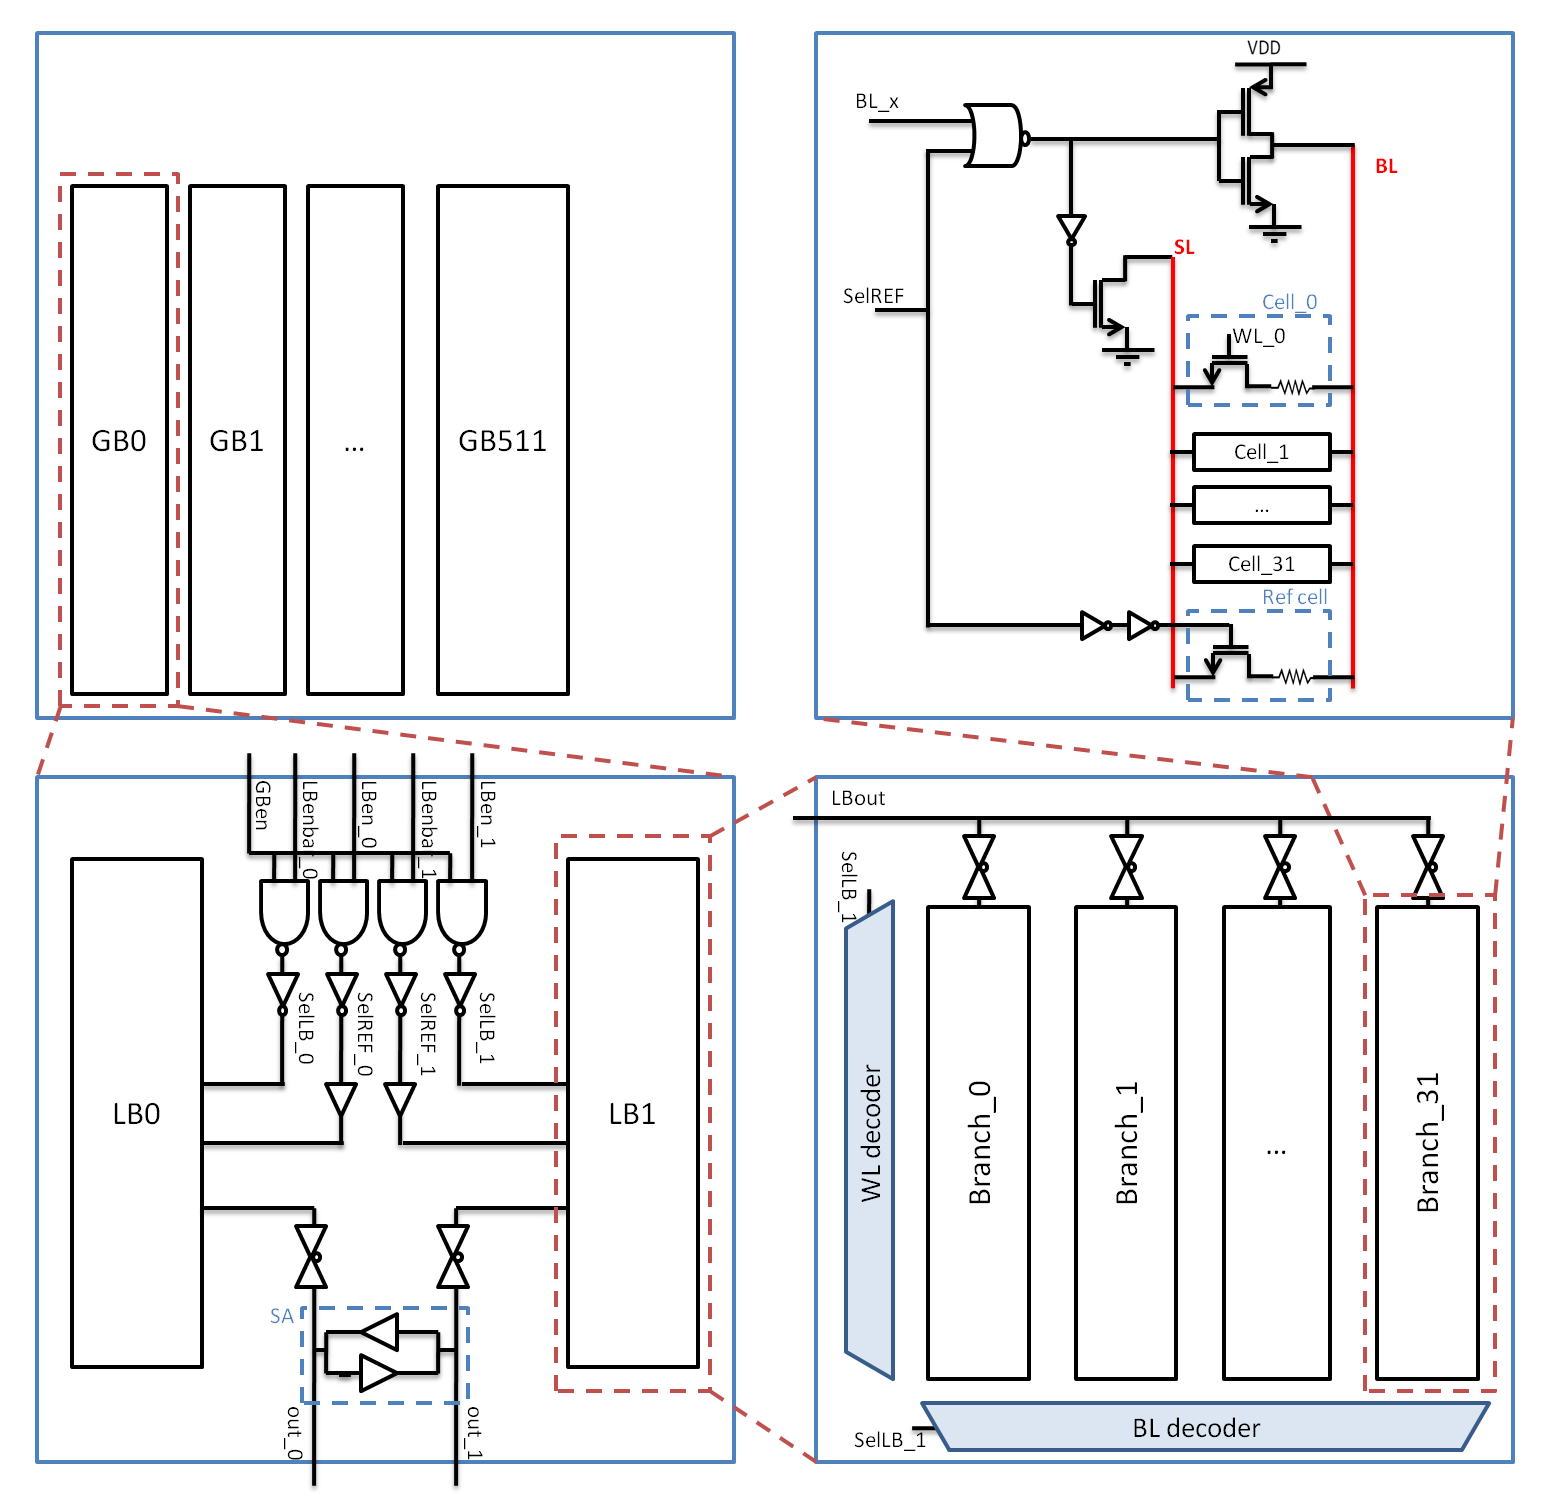
\includegraphics[width=0.5\textwidth]{../fig/paper-architecture.png}
  \caption{Overview architecture}
  \label{fig:architecture}
\end{figure}

\section{Tuning the reference signal distribution}
It is assumed that certain elementary variables of components in the circuit have a normal distribution due to intra-die variations. These variables include the $\Delta_{V_{T}}$ and $\Delta_{\beta}$ parameters of transistors and the $\Delta_{R}$ parameter for the memristor. Due to these elementary variations, signals such as the data and reference signal also have a distribution. The distribution of the reference signal however, can be tuned. Recall that the reference signal is generated by shorting active BLs using passgates. Shorting a BL with an addressed HRS reference cell with a BL with a LRS reference cell would suffice for producing a voltage lying between a HRS data voltage and a LS data voltage. By using this shorting technique however the mean of the reference signal PDF would not lie exactly between the means of the HRS data PDF and LRS data PDF. By implementing more than 2 reference cells for the reference signal, and having more HRS (LRS) cells than LRS (HRS) cells, the mean of the reference signal PDF can be shifted. Furthermore, the distribution will have a smaller spread by implementing a bigger amount of reference cells. One should not implement too many reference cells however, since energy consumption (for each active reference cell, current flows through its corresponding bitline) increases drastically. In this design 16 reference cells in a LB are addressed for generating the reference signal, the remaining 16 serve as dummies. Of the 16 active reference cells, 6 are HRS and 10 are LRS.

\section{Load analysis}
Due to the aforementioned variations in the circuit, the data and reference signals should be designed as such that they are sufficiently far apart. After all the sense amplifier will have an offset voltage because of these same variations and the difference of its inputs must be larger than this offset in order for the SA to latch correctly. Besides designing the SA to have a small offset spread to realize this, the difference of its inputs can be widened by choosing a good load impedance. The load impedance not only influences the value of the data and reference voltages, it also determines the settling time of the charging of the BL and the voltage drop over the memristor. This drop can not be too high, destructive reads might occur because of this. As it turns out, fast settling is not compatible with low memristor voltage drop and large voltage difference. Because the latter are imperative for a functional memory and the former is not, settling time had no bearing on the final choice of load impedance.
Any type of load consisting of minimal length transistors could not produce an equivalent resistance large enough to separate the HRS \& LRS voltage distributions sufficiently. Figure \ref{fig:switchloadresults} shows nominal HRS/LRS voltage differences and memristor voltage drop for several pMOS transistor loads with different sizes. 

\begin{figure}[ht!]
  \centering
  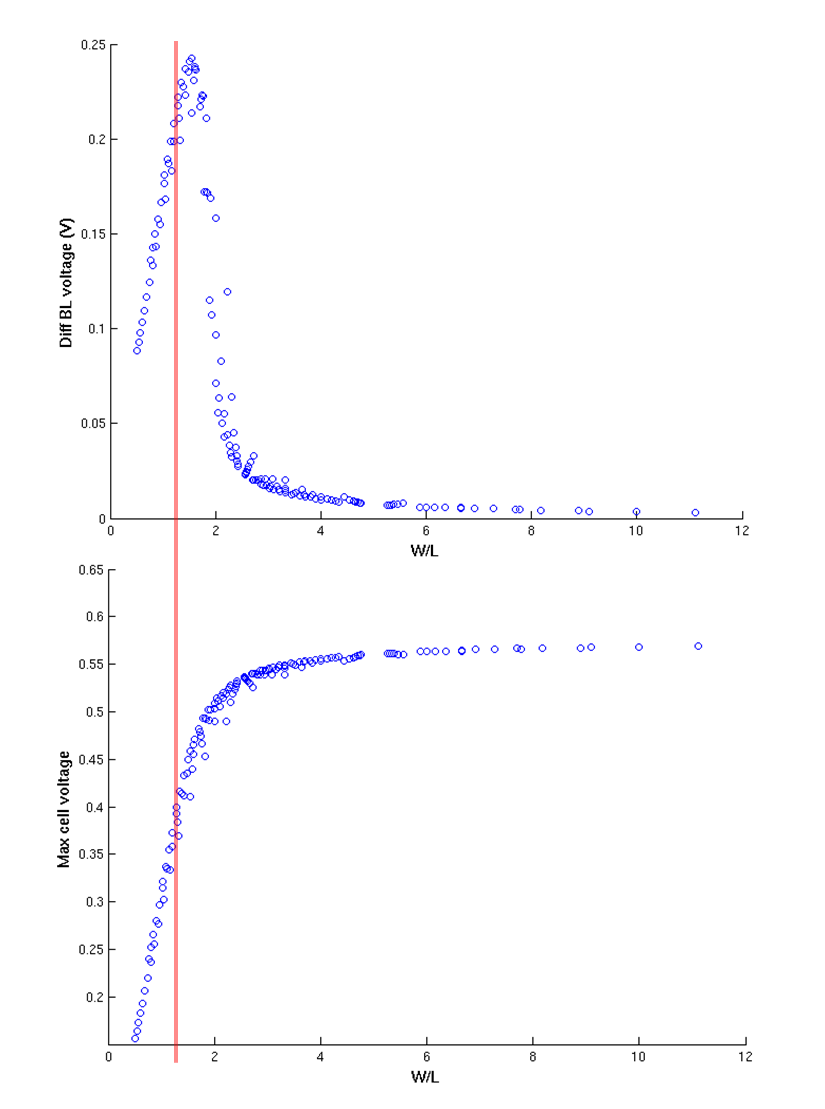
\includegraphics[width=0.5\textwidth]{../fig/hfdst-last-length.png}
  \caption{HRS/LRS voltage difference and memristor voltage drop for pMOS transistor loads}
  \label{fig:switchloadresults}
\end{figure}

In the end a transistor with a width of 300nm and a length of 198nm was chosen. In figure \ref{fig:distributions} the distributions of the data and reference voltages are displayed for this load.


\section{Sense amplifier overlap techniques}
The sense amplifier used in this design is the drain-input latch-type SA (see figure \ref{fig:ourSA}). Its input/output nodes are connected to the output nodes of the local block through complementary passgates. There are two ways to implement the latch timing cycle: one could separate the pass operation from the latch operation or could allow overlap between these two operations.

\begin{figure}[ht!]
  \centering
  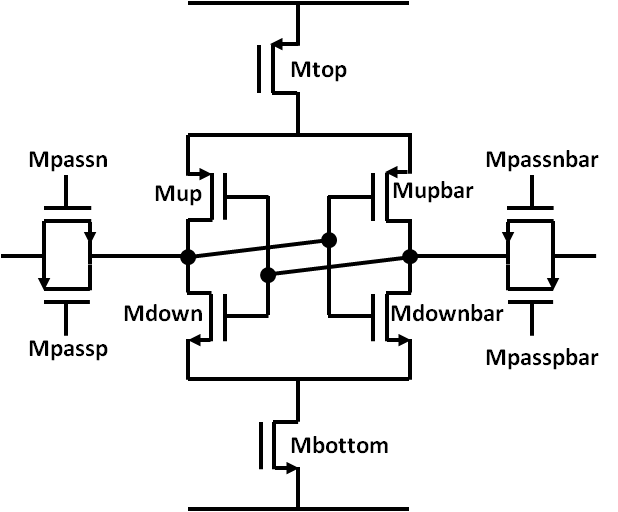
\includegraphics[width=0.25\textwidth]{../fig/hfdstk-sensamp-ourSA.png}
  \caption{Drain-input latch-type sense amplifier used in this design}
  \label{fig:ourSA}
\end{figure}


\subsection{No overlap}
Using this control scheme, the SA would be separated from the local block when enabled. Offset voltage spread is mainly determined by the $\Delta_{V_{T}}$ and $\Delta_{\beta}$ variations of the differential pairs of the SA. These contributions can be decreased by increasing the sizes of the differential pair transistors. Sizing up the top and bottom transistor has not more influence on the latching speed rather than the offset voltage. There is also a maybe slightly surprising contribution on the offset voltage by the passgates. This can be explained by the charge injection of the passgates: when the passgates are turned on, the output voltage of the local block is passed on to the input/output node of the SA almost perfectly - whether there are variations on the transistors or not. When the passgates are turned off, a charge injection occurs on the SA input/output node - distorting the original voltage. The SA operates differentially though, so as long as this charge injection is matched at the two input/output nodes there would be no problem. $\beta$ mismatch of the passgate transistors however results in charge injection mismatch (see figure \ref{fig:chargeinjection}). Hence the contribution of the passgates to the offset voltage spread. This mismatch can be reduced by sizing up the passgates transistors. More charge is injected when the passgates are turned off, but the difference at the two sides is reduced.

\begin{figure}[ht!]
  \centering
  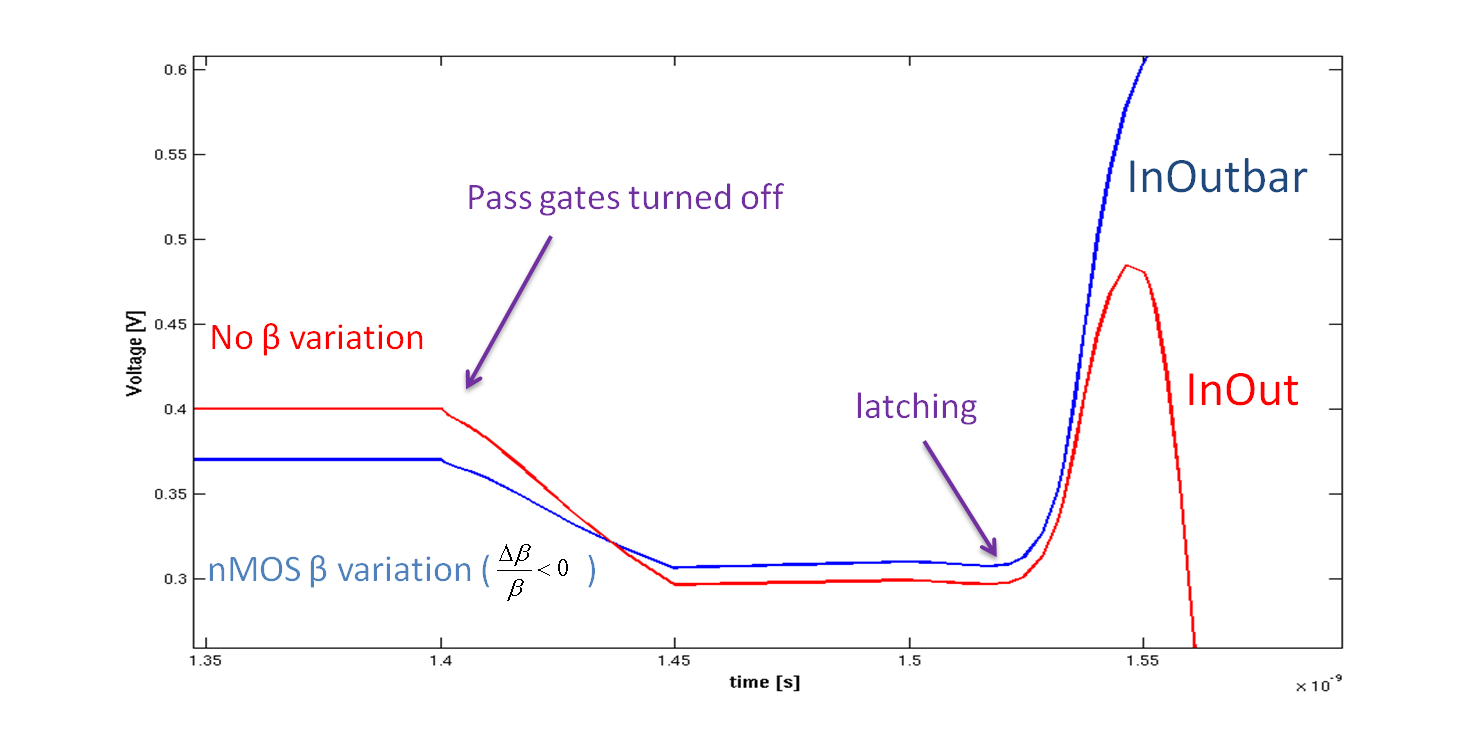
\includegraphics[width=0.5\textwidth]{../fig/hfdstk-sensamp-chargeinjectionmismatch.png}
  \caption{Charge injection mismatch due to $\beta$ variations of passgate transistors}
  \label{fig:chargeinjection}
\end{figure}

\subsection{Overlap}
If the passgates are still turned on when the SA starts latching, the voltage difference of the input/output nodes has not experienced charge injection mismatch. When the voltage difference has been sufficiently amplified, the passgates are turned off. Charge injection (mismatch) will occur, but it will not change the outcome of the latching anymore. During the overlap of the pass and latching operation, the passgates can be modeled by resistors. Neglecting the resistance of the passgates in the local blocks, the situation can be depicted as in figure \ref{fig:RC-latch}. CL is the bitline capacitance.

\begin{figure}[ht!]
  \centering
  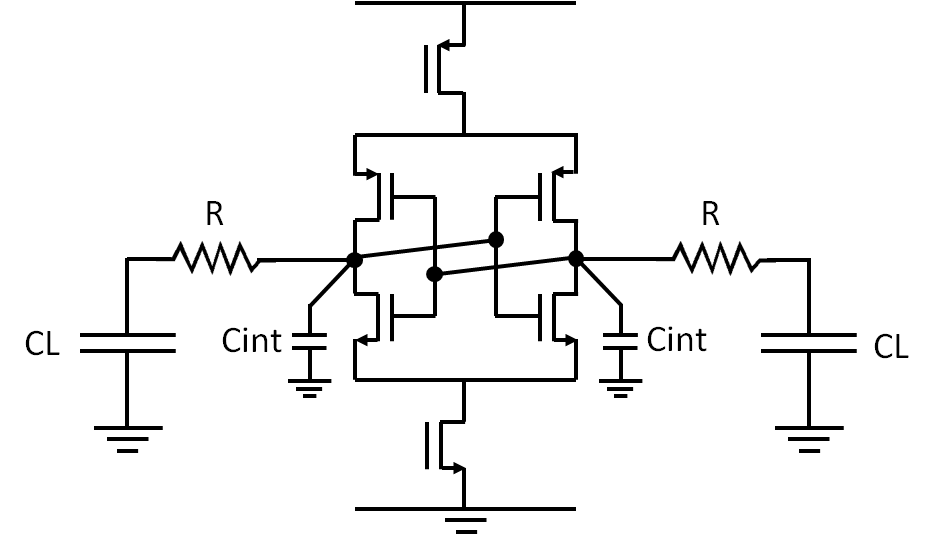
\includegraphics[width=0.25\textwidth]{../fig/hfdstk-sensamp-RC-latch.png}
  \caption{Simplified circuit when overlap between pass enable and latch enable is applied}
  \label{fig:RC-latch}
\end{figure}

One could suspect that a large BL capacitance would significantly increase the latching time. While this is true for small values of R, as can be seen in figure \ref{fig:RC-latch-sim}, for greater values the latching goes through two phases: during the first phase, it appears as if the big capacitance is decoupled from the SA. After this fast phase, settling is much slower. 

\begin{figure}[ht!]
  \centering
  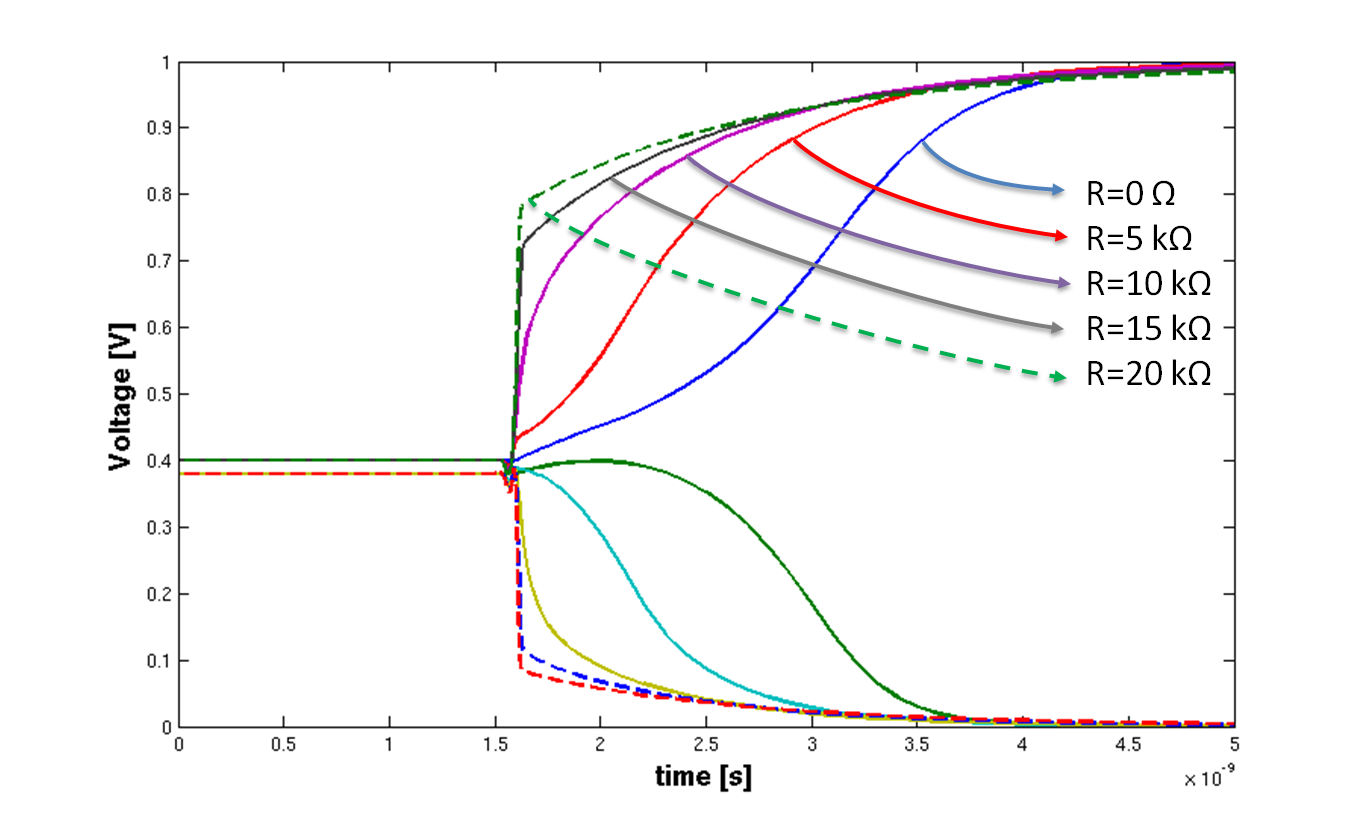
\includegraphics[width=0.5\textwidth]{../fig/hfdstk-sensamp-RC-latch-sim.png}
  \caption{Transient simulation for the schematic of figure \ref{fig:RC-latch} for different values of R, CL = 46fF, SA is minimal, no variations are included in simulation}
  \label{fig:RC-latch-sim}
\end{figure}

This RC-latch effect arises when the RC-product is large. When it occurs, the capacitance behaves as a short-circuit and current flows through the resistor and a corresponding voltage drop over the resistor builds up. Afterwards the load capacitance charges itself at a much lower time constant.

\paragraph{}
The overlap between the enabling of the passgates and the SA thus needn't be this great: a load-less SA latching delay suffices. For this situation $V_{T}$ and $\beta$ mismatch of the ;passgate transistors results in mismatch of the resistors. The interaction between these resistors and the SA is strongly non-linear. Depending on the precharged values of the load capacitances, this R mismatch can result in incorrect latching. There is thus still a contribution of the passgates to the offset voltage spread. The interaction between R and the SA reduces the contributions of the differential pair mismatch however. For a minimal SA, the offset voltage spread is smaller with overlap than without. By sizing all the transistors, this spread can be arbitrarily reduced. The resistance of the passgates mustn't be too small however, or slow settling might occur. Then again, a large SA would probably charge the load capacitance effortlessly anyway.


\section{Read Throughput Results}
A read access time simulation test was performed on the finished circuit (Figure \ref{fig:speedvdd}). In this test the supply voltage was decreased and the maximum read throughput was measured. The test was performed at a (SPICE) temperature of $30^{\circ}\mathrm{C}$. At each point in the shmoo plot, 100 MonteCarlo simulations were performed. The circuit has a read access time of 2.3ns at a supply voltage of 1V. during the read cycle, its energy consumption is 0.51pJ. Most of the energy (65\%) is consumed by the bitlines. 25\% of the energy consumption is due to the logic, the buffers and SA take the remaining 10\%. As the supply voltage goes down, the read throughput also goes down. This is caused by a combination of phenomena. First of all the logic operates slower. This causes a timing issue in which the bitline load transistor is activated before the the cell is. This timing issue results in a rapid increase in bitline voltage which causes a longer settling time of the bitline when the cell is eventually selected. A second reason for the decrease in read throughput at a lower supply voltage, is the slower latching of the SA.

\begin{figure}[h!t]
  \centering
  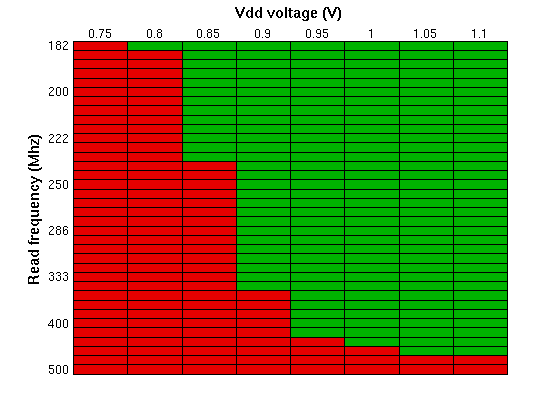
\includegraphics[width=0.5\textwidth]{../fig/hfdst-final-vddspeed.png}
  \caption{Results read access time test}
  \label{fig:speedvdd}
\end{figure}

On figure \ref{fig:speedvdd} it can clearly be seen that the circuit can only operate down to a supply voltage of $0.8V$. An explanation for this is given in figure \ref{fig:vblvdd}. As vdd is decreased, the bitline voltage distributions of the reference signal and HRS \& LRS data signals also decrease. Eventually the bitline voltage distributions overlap and there is a high probability of circuit failure.

\begin{figure}[h!t]
  \centering
  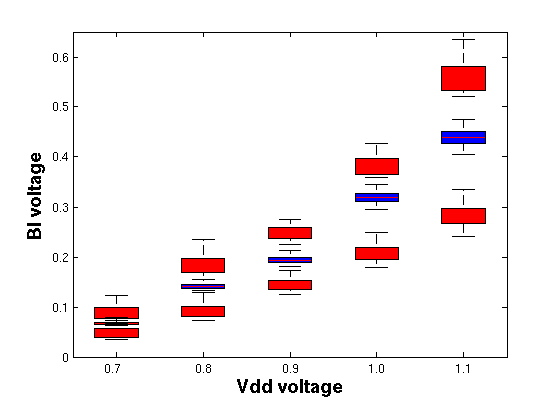
\includegraphics[width=0.5\textwidth]{../fig/hfdst-final-vddbl.png}
  \caption{BL voltage distribution for reference signal and HRS \& LRS signals in function of vdd}
  \label{fig:vblvdd}
\end{figure}
% An example of a floating figure using the graphicx package.
% Note that \label must occur AFTER (or within) \caption.
% For figures, \caption should occur after the \includegraphics.
% Note that IEEEtran v1.7 and later has special internal code that
% is designed to preserve the operation of \label within \caption
% even when the captionsoff option is in effect. However, because
% of issues like this, it may be the safest practice to put all your
% \label just after \caption rather than within \caption{}.
%
% Reminder: the "draftcls" or "draftclsnofoot", not "draft", class
% option should be used if it is desired that the figures are to be
% displayed while in draft mode.
%
%\begin{figure}[!t]
%\centering
%\includegraphics[width=2.5in]{myfigure}
% where an .eps filename suffix will be assumed under latex, 
% and a .pdf suffix will be assumed for pdflatex; or what has been declared
% via \DeclareGraphicsExtensions.
%\caption{Simulation Results.}
%\label{fig_sim}
%\end{figure}

% Note that IEEE typically puts floats only at the top, even when this
% results in a large percentage of a column being occupied by floats.


% An example of a double column floating figure using two subfigures.
% (The subfig.sty package must be loaded for this to work.)
% The subfigure \label commands are set within each subfloat command,
% and the \label for the overall figure must come after \caption.
% \hfil is used as a separator to get equal spacing.
% Watch out that the combined width of all the subfigures on a 
% line do not exceed the text width or a line break will occur.
%
%\begin{figure*}[!t]
%\centering
%\subfloat[Case I]{\includegraphics[width=2.5in]{box}%
%\label{fig_first_case}}
%\hfil
%\subfloat[Case II]{\includegraphics[width=2.5in]{box}%
%\label{fig_second_case}}
%\caption{Simulation results.}
%\label{fig_sim}
%\end{figure*}
%
% Note that often IEEE papers with subfigures do not employ subfigure
% captions (using the optional argument to \subfloat[]), but instead will
% reference/describe all of them (a), (b), etc., within the main caption.


% An example of a floating table. Note that, for IEEE style tables, the 
% \caption command should come BEFORE the table. Table text will default to
% \footnotesize as IEEE normally uses this smaller font for tables.
% The \label must come after \caption as always.
%
%\begin{table}[!t]
%% increase table row spacing, adjust to taste
%\renewcommand{\arraystretch}{1.3}
% if using array.sty, it might be a good idea to tweak the value of
% \extrarowheight as needed to properly center the text within the cells
%\caption{An Example of a Table}
%\label{table_example}
%\centering
%% Some packages, such as MDW tools, offer better commands for making tables
%% than the plain LaTeX2e tabular which is used here.
%\begin{tabular}{|c||c|}
%\hline
%One & Two\\
%\hline
%Three & Four\\
%\hline
%\end{tabular}
%\end{table}


% Note that IEEE does not put floats in the very first column - or typically
% anywhere on the first page for that matter. Also, in-text middle ("here")
% positioning is not used. Most IEEE journals use top floats exclusively.
% Note that, LaTeX2e, unlike IEEE journals, places footnotes above bottom
% floats. This can be corrected via the \fnbelowfloat command of the
% stfloats package.



\section{Conclusion}
A 1Mb RRAM memory has been designed and presented. During the design of this memory, certain techniques were applied to improve performance and reliability. Tuning of the reference voltage distribution was achieved by connecting multiple cells in various states in parallel. A load impedance was carefully chosen to maximize HRS \& LRS voltage differences while keeping the memristor voltage drop sufficiently low. Overlap between passgates and sense amplifier operation reduces offset voltage spread. During this overlap, an RC-latch effect can occur, which decouples the bitline capacitance from the latch for a short time.


% if have a single appendix:
%\appendix[Proof of the Zonklar Equations]
% or
%\appendix  % for no appendix heading
% do not use \section anymore after \appendix, only \section*
% is possibly needed

% use appendices with more than one appendix
% then use \section to start each appendix
% you must declare a \section before using any
% \subsection or using \label (\appendices by itself
% starts a section numbered zero.)
%





% trigger a \newpage just before the given reference
% number - used to balance the columns on the last page
% adjust value as needed - may need to be readjusted if
% the document is modified later
%\IEEEtriggeratref{8}
% The "triggered" command can be changed if desired:
%\IEEEtriggercmd{\enlargethispage{-5in}}

% references section

% can use a bibliography generated by BibTeX as a .bbl file
% BibTeX documentation can be easily obtained at:
% http://www.ctan.org/tex-archive/biblio/bibtex/contrib/doc/
% The IEEEtran BibTeX style support page is at:
% http://www.michaelshell.org/tex/ieeetran/bibtex/
\bibliography{references}{}
\bibliographystyle{IEEEtran}
% argument is your BibTeX string definitions and bibliography database(s)
%\bibliography{IEEEabrv,../bib/paper}


\end{document}


\begin{thebibliography}{0}


\bibitem{sinhuber2012study}
  Study on power and energy demand for sizing the energy storage systems for electrified local public transport buses.
	\hskip 1em plus 0.5em minus 0.4em\relax Sinhuber, Philipp and Rohlfs, Werner and Sauer, Dirk Uwe,
  \emph{Vehicle Power and Propulsion Conference (VPPC), 315--320, 2012}, IEEE.

\end{thebibliography}
%
